\documentclass[10pt]{report}
\usepackage[pdftex]{graphicx}
\usepackage{hyperref}
\hypersetup{ colorlinks=true
           , linkcolor=cyan
           , pdfnewwindow=true 
           }
\usepackage{amsmath}
\usepackage{subfig}
\usepackage{listings}
\usepackage{float}
\newcommand{\HRule}{\rule{\linewidth}{0.5mm}}
\hyphenation{auto-nomous}

% Limited by competition rules to min font size 10 pt, max pages 20

\begin{document}
\title{Rutgers Autonomous Aircraft Team\\Technical Report\\2010 AUVSI UAS Competition}
\author{Patrick Hickey et. al.}
\begin{titlepage}
\begin{center}

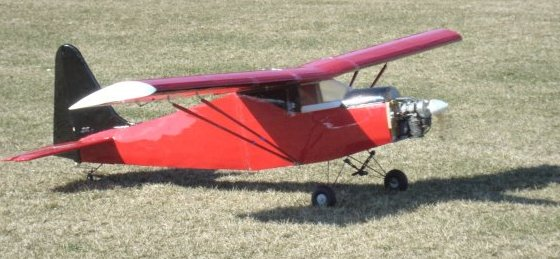
\includegraphics[width=0.5\textwidth]{../images/daedalus.jpg}\\[1cm]
\HRule \\[1cm]
{ \huge \bfseries Rutgers University Autonomous Aircraft Team } \\[0.5cm]
\HRule \\[0.5cm]
{ \large \bfseries Technical Report }
\\[0.5cm]
{ \large \bfseries 2010 AUVSI UAS Competition }
\\[0.5cm]
\HRule \\[1cm]

  {\large Amanda Gaetano, Anthony Garrison, Pat Hickey,}
\\{\large Stephen Indyk, Cogan Noll, John Palmer,}
\\{\large Adrien Perkins, Gregory Quinn, and Michael Varga}
\\[1cm]
\emph{Thank you to our sponsors}
\\ Rutgers University Engineering Governance Council
\\ Rutgers Alumni Association
\\ WINLAB
\\ Invensense, Inc.
\\ ST Micro, Inc.

\vfill
{\large \today}

\end{center}
\end{titlepage}


\begin{abstract}
We will write the abstract after the rest of the paper is finished. If we're really close to the page limit, we may be able to omit it.
\end{abstract}

\section{Introduction}

Brief overview of what we accomplished. This should be a very brief chronology of the engineering we've done to date.

\section{Systems Engineering}
The main systems engineering approach that was used in order to finish construction of the planes efficiently and in a timely manner was to break the team into two main groups: the mechanical team and the electronics team.  The mechanical team was in charge of the rebuild and build process of the \emph{Daedalus} and the \emph{Knight Two}, respectively.  In order to maximize efficiency we further divided the mechanical team into sub groups placing members where they were best suited.  During both constructions we split into a wing and tail section group and a fuselage group.  While all the construction was going on, two expert builders from the local R/C club would come and advise us when we were unsure how to proceed in order to have the best balance of weight and strength.  Along with the actual construction of the planes, the mechanical team also focused on modifying the structures of the planes in order to fit the desired payload: the autopilot system and the imaging system.

The electronics team was in charge of the autopilot system and the imaging system.  Originally a large and heavy system was to be used for an imaging system, but as the year progress a lighter and smaller alternative was found, which helped the mechanical team in the placement of the imaging system…(I do not know the details of what they did, that’s all Pat)


We will be performing a manual take off, and giving the autopilot system control of the aircraft once the plane is in the air.  For landing, we will do the same process in reverse, and land the plane manually.



%One thing we need is a good justification for having built two fucking giant airframes. Lets point out that we initially assumed a much heavier payload, but found lighter and smaller alternatives as the year went on. We decided it was better to be too big than too small. A large plane with lower wing loading would be easier to control, and easier to recover in case power is lost. (someone check that math)

\section{Flight Vehicle}

At the time of this writing, we have completed and flown a single flight vehicle, which we have named the \emph{Daedalus}.
We have also nearly completed a very similar backup airframe which serve as a backup in case the \emph{Daedalus} has a disaster. The \emph{Knight Two} will be fitted with 

\subsection{Airframe}

We elected to persue a kit-type airplane rather than our own design. 
Our own custom design, the \emph{Icarus}, suffered a catastrophic structural failure last year. From this, we learned that custom structures require much more testing and revision than a proven kit. We also reconsidered our payload requirments and decided we could easily modify a kit plane to accept our autopilot and imaging system.

\subsubsection{Daedalus}

A member of our local R/C club, Tri-County RC \cite{tricountyRC}, donated a ten-foot wingspan high wing trainer to our club. The plane, first built out of foam and balsa from long-lost plans in 1986, was accepted graciously, but required quite a bit of work before it was once again flightworthy. We removed the covering to find water damage and rot which resulted from years of storage. We stripped and rebuilt nearly the entire airframe, adding carbon-fiber reinforcements to the wing in anticipation of increased wing loading due to our payload.


Once rebuilt and covered, we tested the \emph{Daedalus} in our shop to ensure the rebuilt structure was strong enough. Of particular concern was interface between the wings and the center section---it was important to confirm that the wings were mounted and reinforced in a manner that would permit them to carry the load of the plane while in flight.  To this end, we put the \emph{Daedalus} through a series of static and dynamic ``sandbag tests.''  The plane was carefully supported under the center section, nose, and tail while pre-weighted bags of sand were slowly placed symetrically and simultaneously on the underside of each wing, starting from the innermost rib.  The \emph{Daedalus} easily supported XX lbs (XX percent of its weight) under static loading.  We then lifted the plane off its supports and jostled it to simulate in-flight motion.  The plane seemed to remain stable, and upon further observation after unloading, no cracks or defects were detected.


Satisfied, we proceeded through the usual engine and surface tests before taxiing the plane around a parking lot.  We brought the plane back inside, examined it for signs of stress and, finding everything in good condition, deemed the \emph{Daedalus} ready to fly.


Figure goes here: Photos of Daedalus in construction, sandbag testing

Someone please detail the outer dimensions. The inner dimensions, space used for flight electronics, space used for payload underneath. Landing gear height. Number of servos and their locations

Figure may go here: Line drawing of Daedalus. JOHN

\subsubsection{Knight Two}

In order to mitigate a disaster such as we had last year, we decided to build another airframe which could replace the \emph{Daedalus} at short notice. We selected an Aero-Design 12 Foot Telemaster \cite{aerodesign} because it was available as a balsa kit and similar in size to the \emph{Daedalus}.

We named it the \emph{Knight Two} after the Rutgers University mascot, the Scarlet Knight. We may rename it if someone can think of a better name. Pat needed to think up a decent name real fast in order to make this rough draft.

Since our testing plan for the \emph{Daedalus} was successful, we will follow the same plan when, in the coming weeks, we finish building \emph{Knight Two}.

Figure goes here: Photos of Knight Two in construction, sandbag testing

Someone please detail the outer dimensions. The inner dimensions, space used for flight electronics, space used for payload underneath. Landing gear height. Number of servos and their locations

Figure may go here: Line drawing of Knight Two. JOHN

\subsection{Power}

\subsubsection{Engine}

Each airframe has a 45cc gasoline engine. Each airframe has a xx ounce gasoline tank. Based on our flight tests, with climbs to 400 feet AGL, a full xx ounce gasoline tank gives us xx minutes of flight time. (can someone guestimate this? Do we have data from break-in, etc)

\subsubsection{Batteries}

Each airframe has nearly identical flight electronics. To power a Futaba 2.4GHz receiver and 6 servos for a XX minute flight, we selected a 2 cell XX amp hour Lithium Ion battery with a 5v, 10A capacity switching regulator made by Castle Creations. Pat will add more here if he has to.

\section{Autopilot}
Our entry uses an autopilot system based off the open source 
Paparazzi project\cite{paparazziweb}. 
We ported the airborne code to Linux in order to use a single computer for all of our flight hardware and software.

\subsection{Requirments}

We needed to interface with the following hardware components:
\begin{itemize}
	\item GPS
	\item servos
	\item camera
	\item etc.
\end{itemize}

Interfacing with such a large array of devices meant we had to use a ...

\subsection{Hardware}
Single board computer: beagleboard.

Description of each input, output interface.

Figure goes here: Hardware connection diagram. PAT
\subsection{Software}
PAT

Figure goes here: interprocess communication. PAT
\subsection{Ground Station}
Because we based our autopilot software on the Paparazzi project, we were able to make use of their excellent ground control software (GCS) with essentially no modifications.

Detail the capabilities of the Paparazzi GCS.

Figure goes here: Paparazzi ground station screenshot, or whatever. 
\subsection{Tuning and Testing}
PAT

\section{Imaging System}

To obtain images of targets in flight we have created an Imaging System capable of meeting all the requirements of the competition.  The system consists of a pan-tilt camera on the plane, communication software on the plane, and our ``Image Station'' application running on a dedicated laptop.  The Image Station communicates with the plane in real time via two different sets of wireless radios.  Using the Image Station, the operator can view a live video stream from the plane, control the pan-tilt camera remotely, and download and manipulate images.

\subsection{Camera}

MICHAEL : physical specification of camera (size, 5 megapixel stills). We selected it because...

MICHAEL: camera interfaces: serial and USB 

The camera will be mounted in a pan and tilt unit, which will ... STEVE, PAT

\subsection{Obtaining Images}

The entire imaging system is controlled by the ``Image Station Operator''.  They view a live video stream coming from the camera on the plane, which is transmitted over a high bandwidth radio.  The operator can also control the camera by sending commands to the plane over an Xbee Radio link.  In order to assist the operator in finding targets, a target locating algorithm will be run on the video feed to highlight possible targets.  At the time of writing work is in progress on this feature, and it is being implemented using the OpenCV library \cite{opencv} with contour detection and polygonal mapping functions.

\begin{figure} [H]
  \centering
  	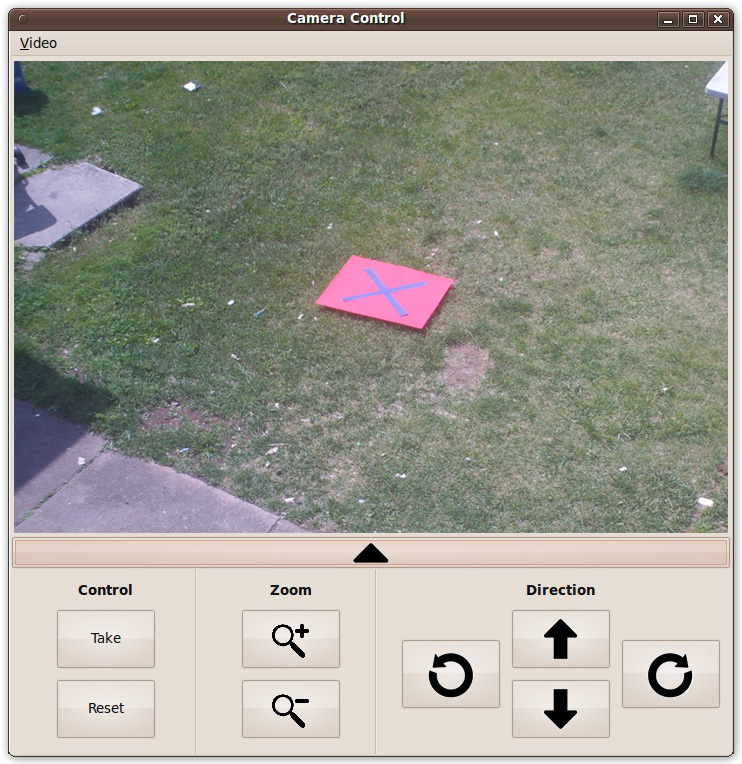
\includegraphics[width=0.9\textwidth]{../images/ImageStationControls.jpg}
  	\caption[Image Station Control Panel]{The Control Panel for the Image Station.  Above is a live video feed from the plane.  Below are controls to adjust the pan/tilt of the unit, zoom in/out, take a picture, and reset the camera to a neutral position.}
  	\label{imagestationcontrols}
\end{figure}

When a picture is taken on the plane it is immediately saved on the camera's memory card.  In order to view that picture on the ground it must first be transferred to the plane's main computer (beagle board), and then downloaded to the Image Station over the Xbee connection.

\subsection{Downloading Images in Real Time}

Once images are on the plane's computer they are ready to be downloaded over the Xbee Radio link.  Each image is fairly large, and our bandwidth is only around 115200 baud, so we use a bandwidth conserving method to transfer images.  The entire image is first downloaded as a low-res `thumbnail.'  Once that is available for viewing, the operator can select an area of interest and download a high-res crop of just that area.  This allows us to quickly obtain high resolution images of the targets of interest.

\begin{figure} [h]
  \centering
  	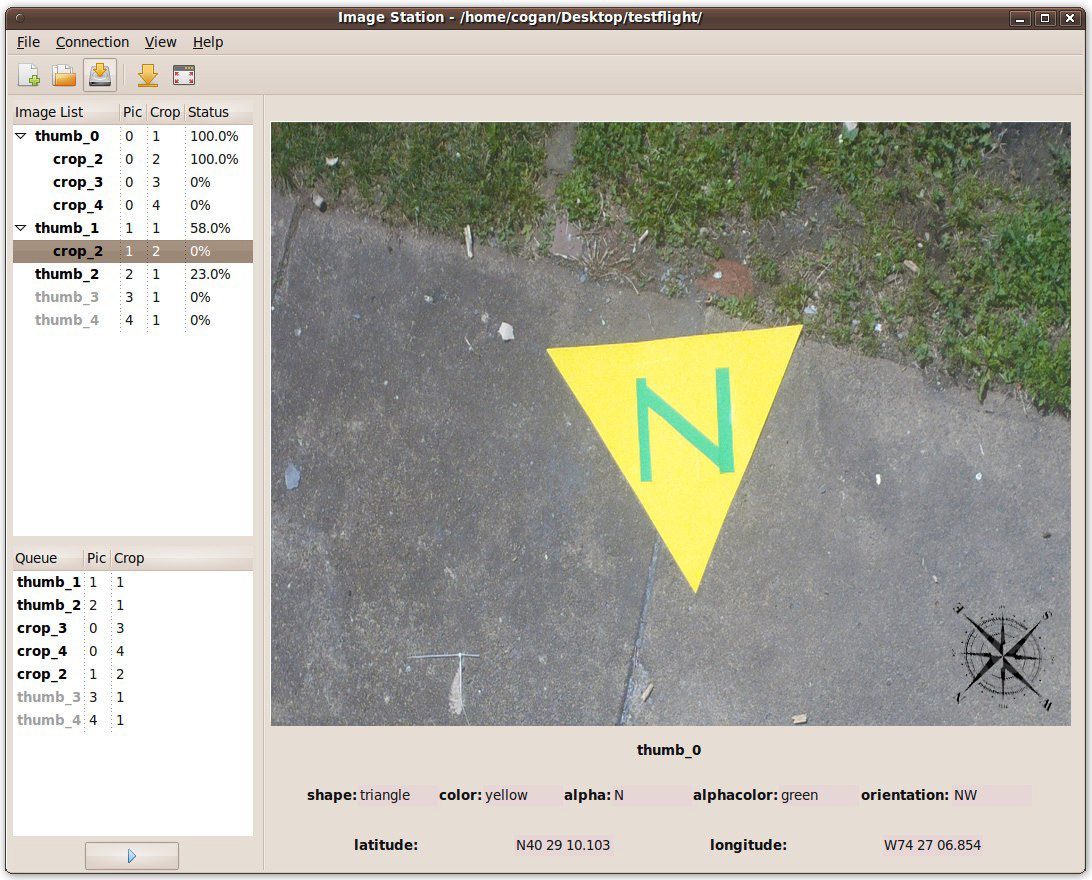
\includegraphics[width=0.9\textwidth]{../images/ImageStationMain.jpg}
  	\caption[Image Station Interface]{The main interface for the Image Station.  All the images that have been taken are displayed on the top left.  The queue of images to download is on the bottom left.  On the right is the currently displayed image, with target information underneath.}
  	\label{imagestationinterface}
\end{figure}

\subsection{Identifying target characteristics}

When an image has been fully downloaded to the ground targets can be identified and tagged with metadata.  Information about the plane's orientation, gps coordinates, altitude, yaw/pitch/roll, and pan/tilt of the camera are sent down with the image.  Using this information the GPS location of the target can be determined using the intrinsic properties of the camera and some basic trigonometry. target shape, color, alphanumeric, alphanumeric color, and orienttion are all entered manually by the operator.

\section{Operation Safety}

We consider the safety of our team, our aircraft, and our spectators to be of utmost importance.  As such, we've implemented numerous safety features and developed a strict procedure for starting, taxiing, and flying the plane.  This procedure enables us to ensure that all personnel are safely in place, and that no intergral checks are missed.

\subsection{Safety Features}
Our system is designed to gracefully handle any failure while continuing to ensure the safety of those nearby.
\begin{itemize}
\item Channel 5 (?) allows quick switch to safety pilot in case of autopilot malfunction
\item autopilot return home command if connection is lost (I presume it does something like that?)
\item kill switch
\item etc?
\end{itemize}

\subsection{Procedures}
Our team employs a clearly defined flight routine every time the engine is started.  Blah blah blah.  Maybe just include either the flight routine or pre-flight checklist as an appendix?  I feel like this stuff is pretty standard, and there's probably no point in us wasting a lot of space rambling about it.  


\bibliographystyle{plain}
\bibliography{paper}

\end{document}
